\documentclass{article} % For LaTeX2e
\usepackage{iclr2022_conference,times}
% Optional math commands from https://github.com/goodfeli/dlbook_notation.
%%%%% NEW MATH DEFINITIONS %%%%%

\usepackage{amsmath,amsfonts,bm}

% Mark sections of captions for referring to divisions of figures
\newcommand{\figleft}{{\em (Left)}}
\newcommand{\figcenter}{{\em (Center)}}
\newcommand{\figright}{{\em (Right)}}
\newcommand{\figtop}{{\em (Top)}}
\newcommand{\figbottom}{{\em (Bottom)}}
\newcommand{\captiona}{{\em (a)}}
\newcommand{\captionb}{{\em (b)}}
\newcommand{\captionc}{{\em (c)}}
\newcommand{\captiond}{{\em (d)}}

% Highlight a newly defined term
\newcommand{\newterm}[1]{{\bf #1}}


% Figure reference, lower-case.
\def\figref#1{figure~\ref{#1}}
% Figure reference, capital. For start of sentence
\def\Figref#1{Figure~\ref{#1}}
\def\twofigref#1#2{figures \ref{#1} and \ref{#2}}
\def\quadfigref#1#2#3#4{figures \ref{#1}, \ref{#2}, \ref{#3} and \ref{#4}}
% Section reference, lower-case.
\def\secref#1{section~\ref{#1}}
% Section reference, capital.
\def\Secref#1{Section~\ref{#1}}
% Reference to two sections.
\def\twosecrefs#1#2{sections \ref{#1} and \ref{#2}}
% Reference to three sections.
\def\secrefs#1#2#3{sections \ref{#1}, \ref{#2} and \ref{#3}}
% Reference to an equation, lower-case.
\def\eqref#1{equation~\ref{#1}}
% Reference to an equation, upper case
\def\Eqref#1{Equation~\ref{#1}}
% A raw reference to an equation---avoid using if possible
\def\plaineqref#1{\ref{#1}}
% Reference to a chapter, lower-case.
\def\chapref#1{chapter~\ref{#1}}
% Reference to an equation, upper case.
\def\Chapref#1{Chapter~\ref{#1}}
% Reference to a range of chapters
\def\rangechapref#1#2{chapters\ref{#1}--\ref{#2}}
% Reference to an algorithm, lower-case.
\def\algref#1{algorithm~\ref{#1}}
% Reference to an algorithm, upper case.
\def\Algref#1{Algorithm~\ref{#1}}
\def\twoalgref#1#2{algorithms \ref{#1} and \ref{#2}}
\def\Twoalgref#1#2{Algorithms \ref{#1} and \ref{#2}}
% Reference to a part, lower case
\def\partref#1{part~\ref{#1}}
% Reference to a part, upper case
\def\Partref#1{Part~\ref{#1}}
\def\twopartref#1#2{parts \ref{#1} and \ref{#2}}

\def\ceil#1{\lceil #1 \rceil}
\def\floor#1{\lfloor #1 \rfloor}
\def\1{\bm{1}}
\newcommand{\train}{\mathcal{D}}
\newcommand{\valid}{\mathcal{D_{\mathrm{valid}}}}
\newcommand{\test}{\mathcal{D_{\mathrm{test}}}}

\def\eps{{\epsilon}}


% Random variables
\def\reta{{\textnormal{$\eta$}}}
\def\ra{{\textnormal{a}}}
\def\rb{{\textnormal{b}}}
\def\rc{{\textnormal{c}}}
\def\rd{{\textnormal{d}}}
\def\re{{\textnormal{e}}}
\def\rf{{\textnormal{f}}}
\def\rg{{\textnormal{g}}}
\def\rh{{\textnormal{h}}}
\def\ri{{\textnormal{i}}}
\def\rj{{\textnormal{j}}}
\def\rk{{\textnormal{k}}}
\def\rl{{\textnormal{l}}}
% rm is already a command, just don't name any random variables m
\def\rn{{\textnormal{n}}}
\def\ro{{\textnormal{o}}}
\def\rp{{\textnormal{p}}}
\def\rq{{\textnormal{q}}}
\def\rr{{\textnormal{r}}}
\def\rs{{\textnormal{s}}}
\def\rt{{\textnormal{t}}}
\def\ru{{\textnormal{u}}}
\def\rv{{\textnormal{v}}}
\def\rw{{\textnormal{w}}}
\def\rx{{\textnormal{x}}}
\def\ry{{\textnormal{y}}}
\def\rz{{\textnormal{z}}}

% Random vectors
\def\rvepsilon{{\mathbf{\epsilon}}}
\def\rvtheta{{\mathbf{\theta}}}
\def\rva{{\mathbf{a}}}
\def\rvb{{\mathbf{b}}}
\def\rvc{{\mathbf{c}}}
\def\rvd{{\mathbf{d}}}
\def\rve{{\mathbf{e}}}
\def\rvf{{\mathbf{f}}}
\def\rvg{{\mathbf{g}}}
\def\rvh{{\mathbf{h}}}
\def\rvu{{\mathbf{i}}}
\def\rvj{{\mathbf{j}}}
\def\rvk{{\mathbf{k}}}
\def\rvl{{\mathbf{l}}}
\def\rvm{{\mathbf{m}}}
\def\rvn{{\mathbf{n}}}
\def\rvo{{\mathbf{o}}}
\def\rvp{{\mathbf{p}}}
\def\rvq{{\mathbf{q}}}
\def\rvr{{\mathbf{r}}}
\def\rvs{{\mathbf{s}}}
\def\rvt{{\mathbf{t}}}
\def\rvu{{\mathbf{u}}}
\def\rvv{{\mathbf{v}}}
\def\rvw{{\mathbf{w}}}
\def\rvx{{\mathbf{x}}}
\def\rvy{{\mathbf{y}}}
\def\rvz{{\mathbf{z}}}

% Elements of random vectors
\def\erva{{\textnormal{a}}}
\def\ervb{{\textnormal{b}}}
\def\ervc{{\textnormal{c}}}
\def\ervd{{\textnormal{d}}}
\def\erve{{\textnormal{e}}}
\def\ervf{{\textnormal{f}}}
\def\ervg{{\textnormal{g}}}
\def\ervh{{\textnormal{h}}}
\def\ervi{{\textnormal{i}}}
\def\ervj{{\textnormal{j}}}
\def\ervk{{\textnormal{k}}}
\def\ervl{{\textnormal{l}}}
\def\ervm{{\textnormal{m}}}
\def\ervn{{\textnormal{n}}}
\def\ervo{{\textnormal{o}}}
\def\ervp{{\textnormal{p}}}
\def\ervq{{\textnormal{q}}}
\def\ervr{{\textnormal{r}}}
\def\ervs{{\textnormal{s}}}
\def\ervt{{\textnormal{t}}}
\def\ervu{{\textnormal{u}}}
\def\ervv{{\textnormal{v}}}
\def\ervw{{\textnormal{w}}}
\def\ervx{{\textnormal{x}}}
\def\ervy{{\textnormal{y}}}
\def\ervz{{\textnormal{z}}}

% Random matrices
\def\rmA{{\mathbf{A}}}
\def\rmB{{\mathbf{B}}}
\def\rmC{{\mathbf{C}}}
\def\rmD{{\mathbf{D}}}
\def\rmE{{\mathbf{E}}}
\def\rmF{{\mathbf{F}}}
\def\rmG{{\mathbf{G}}}
\def\rmH{{\mathbf{H}}}
\def\rmI{{\mathbf{I}}}
\def\rmJ{{\mathbf{J}}}
\def\rmK{{\mathbf{K}}}
\def\rmL{{\mathbf{L}}}
\def\rmM{{\mathbf{M}}}
\def\rmN{{\mathbf{N}}}
\def\rmO{{\mathbf{O}}}
\def\rmP{{\mathbf{P}}}
\def\rmQ{{\mathbf{Q}}}
\def\rmR{{\mathbf{R}}}
\def\rmS{{\mathbf{S}}}
\def\rmT{{\mathbf{T}}}
\def\rmU{{\mathbf{U}}}
\def\rmV{{\mathbf{V}}}
\def\rmW{{\mathbf{W}}}
\def\rmX{{\mathbf{X}}}
\def\rmY{{\mathbf{Y}}}
\def\rmZ{{\mathbf{Z}}}

% Elements of random matrices
\def\ermA{{\textnormal{A}}}
\def\ermB{{\textnormal{B}}}
\def\ermC{{\textnormal{C}}}
\def\ermD{{\textnormal{D}}}
\def\ermE{{\textnormal{E}}}
\def\ermF{{\textnormal{F}}}
\def\ermG{{\textnormal{G}}}
\def\ermH{{\textnormal{H}}}
\def\ermI{{\textnormal{I}}}
\def\ermJ{{\textnormal{J}}}
\def\ermK{{\textnormal{K}}}
\def\ermL{{\textnormal{L}}}
\def\ermM{{\textnormal{M}}}
\def\ermN{{\textnormal{N}}}
\def\ermO{{\textnormal{O}}}
\def\ermP{{\textnormal{P}}}
\def\ermQ{{\textnormal{Q}}}
\def\ermR{{\textnormal{R}}}
\def\ermS{{\textnormal{S}}}
\def\ermT{{\textnormal{T}}}
\def\ermU{{\textnormal{U}}}
\def\ermV{{\textnormal{V}}}
\def\ermW{{\textnormal{W}}}
\def\ermX{{\textnormal{X}}}
\def\ermY{{\textnormal{Y}}}
\def\ermZ{{\textnormal{Z}}}

% Vectors
\def\vzero{{\bm{0}}}
\def\vone{{\bm{1}}}
\def\vmu{{\bm{\mu}}}
\def\vtheta{{\bm{\theta}}}
\def\va{{\bm{a}}}
\def\vb{{\bm{b}}}
\def\vc{{\bm{c}}}
\def\vd{{\bm{d}}}
\def\ve{{\bm{e}}}
\def\vf{{\bm{f}}}
\def\vg{{\bm{g}}}
\def\vh{{\bm{h}}}
\def\vi{{\bm{i}}}
\def\vj{{\bm{j}}}
\def\vk{{\bm{k}}}
\def\vl{{\bm{l}}}
\def\vm{{\bm{m}}}
\def\vn{{\bm{n}}}
\def\vo{{\bm{o}}}
\def\vp{{\bm{p}}}
\def\vq{{\bm{q}}}
\def\vr{{\bm{r}}}
\def\vs{{\bm{s}}}
\def\vt{{\bm{t}}}
\def\vu{{\bm{u}}}
\def\vv{{\bm{v}}}
\def\vw{{\bm{w}}}
\def\vx{{\bm{x}}}
\def\vy{{\bm{y}}}
\def\vz{{\bm{z}}}

% Elements of vectors
\def\evalpha{{\alpha}}
\def\evbeta{{\beta}}
\def\evepsilon{{\epsilon}}
\def\evlambda{{\lambda}}
\def\evomega{{\omega}}
\def\evmu{{\mu}}
\def\evpsi{{\psi}}
\def\evsigma{{\sigma}}
\def\evtheta{{\theta}}
\def\eva{{a}}
\def\evb{{b}}
\def\evc{{c}}
\def\evd{{d}}
\def\eve{{e}}
\def\evf{{f}}
\def\evg{{g}}
\def\evh{{h}}
\def\evi{{i}}
\def\evj{{j}}
\def\evk{{k}}
\def\evl{{l}}
\def\evm{{m}}
\def\evn{{n}}
\def\evo{{o}}
\def\evp{{p}}
\def\evq{{q}}
\def\evr{{r}}
\def\evs{{s}}
\def\evt{{t}}
\def\evu{{u}}
\def\evv{{v}}
\def\evw{{w}}
\def\evx{{x}}
\def\evy{{y}}
\def\evz{{z}}

% Matrix
\def\mA{{\bm{A}}}
\def\mB{{\bm{B}}}
\def\mC{{\bm{C}}}
\def\mD{{\bm{D}}}
\def\mE{{\bm{E}}}
\def\mF{{\bm{F}}}
\def\mG{{\bm{G}}}
\def\mH{{\bm{H}}}
\def\mI{{\bm{I}}}
\def\mJ{{\bm{J}}}
\def\mK{{\bm{K}}}
\def\mL{{\bm{L}}}
\def\mM{{\bm{M}}}
\def\mN{{\bm{N}}}
\def\mO{{\bm{O}}}
\def\mP{{\bm{P}}}
\def\mQ{{\bm{Q}}}
\def\mR{{\bm{R}}}
\def\mS{{\bm{S}}}
\def\mT{{\bm{T}}}
\def\mU{{\bm{U}}}
\def\mV{{\bm{V}}}
\def\mW{{\bm{W}}}
\def\mX{{\bm{X}}}
\def\mY{{\bm{Y}}}
\def\mZ{{\bm{Z}}}
\def\mBeta{{\bm{\beta}}}
\def\mPhi{{\bm{\Phi}}}
\def\mLambda{{\bm{\Lambda}}}
\def\mSigma{{\bm{\Sigma}}}

% Tensor
\DeclareMathAlphabet{\mathsfit}{\encodingdefault}{\sfdefault}{m}{sl}
\SetMathAlphabet{\mathsfit}{bold}{\encodingdefault}{\sfdefault}{bx}{n}
\newcommand{\tens}[1]{\bm{\mathsfit{#1}}}
\def\tA{{\tens{A}}}
\def\tB{{\tens{B}}}
\def\tC{{\tens{C}}}
\def\tD{{\tens{D}}}
\def\tE{{\tens{E}}}
\def\tF{{\tens{F}}}
\def\tG{{\tens{G}}}
\def\tH{{\tens{H}}}
\def\tI{{\tens{I}}}
\def\tJ{{\tens{J}}}
\def\tK{{\tens{K}}}
\def\tL{{\tens{L}}}
\def\tM{{\tens{M}}}
\def\tN{{\tens{N}}}
\def\tO{{\tens{O}}}
\def\tP{{\tens{P}}}
\def\tQ{{\tens{Q}}}
\def\tR{{\tens{R}}}
\def\tS{{\tens{S}}}
\def\tT{{\tens{T}}}
\def\tU{{\tens{U}}}
\def\tV{{\tens{V}}}
\def\tW{{\tens{W}}}
\def\tX{{\tens{X}}}
\def\tY{{\tens{Y}}}
\def\tZ{{\tens{Z}}}


% Graph
\def\gA{{\mathcal{A}}}
\def\gB{{\mathcal{B}}}
\def\gC{{\mathcal{C}}}
\def\gD{{\mathcal{D}}}
\def\gE{{\mathcal{E}}}
\def\gF{{\mathcal{F}}}
\def\gG{{\mathcal{G}}}
\def\gH{{\mathcal{H}}}
\def\gI{{\mathcal{I}}}
\def\gJ{{\mathcal{J}}}
\def\gK{{\mathcal{K}}}
\def\gL{{\mathcal{L}}}
\def\gM{{\mathcal{M}}}
\def\gN{{\mathcal{N}}}
\def\gO{{\mathcal{O}}}
\def\gP{{\mathcal{P}}}
\def\gQ{{\mathcal{Q}}}
\def\gR{{\mathcal{R}}}
\def\gS{{\mathcal{S}}}
\def\gT{{\mathcal{T}}}
\def\gU{{\mathcal{U}}}
\def\gV{{\mathcal{V}}}
\def\gW{{\mathcal{W}}}
\def\gX{{\mathcal{X}}}
\def\gY{{\mathcal{Y}}}
\def\gZ{{\mathcal{Z}}}

% Sets
\def\sA{{\mathbb{A}}}
\def\sB{{\mathbb{B}}}
\def\sC{{\mathbb{C}}}
\def\sD{{\mathbb{D}}}
% Don't use a set called E, because this would be the same as our symbol
% for expectation.
\def\sF{{\mathbb{F}}}
\def\sG{{\mathbb{G}}}
\def\sH{{\mathbb{H}}}
\def\sI{{\mathbb{I}}}
\def\sJ{{\mathbb{J}}}
\def\sK{{\mathbb{K}}}
\def\sL{{\mathbb{L}}}
\def\sM{{\mathbb{M}}}
\def\sN{{\mathbb{N}}}
\def\sO{{\mathbb{O}}}
\def\sP{{\mathbb{P}}}
\def\sQ{{\mathbb{Q}}}
\def\sR{{\mathbb{R}}}
\def\sS{{\mathbb{S}}}
\def\sT{{\mathbb{T}}}
\def\sU{{\mathbb{U}}}
\def\sV{{\mathbb{V}}}
\def\sW{{\mathbb{W}}}
\def\sX{{\mathbb{X}}}
\def\sY{{\mathbb{Y}}}
\def\sZ{{\mathbb{Z}}}

% Entries of a matrix
\def\emLambda{{\Lambda}}
\def\emA{{A}}
\def\emB{{B}}
\def\emC{{C}}
\def\emD{{D}}
\def\emE{{E}}
\def\emF{{F}}
\def\emG{{G}}
\def\emH{{H}}
\def\emI{{I}}
\def\emJ{{J}}
\def\emK{{K}}
\def\emL{{L}}
\def\emM{{M}}
\def\emN{{N}}
\def\emO{{O}}
\def\emP{{P}}
\def\emQ{{Q}}
\def\emR{{R}}
\def\emS{{S}}
\def\emT{{T}}
\def\emU{{U}}
\def\emV{{V}}
\def\emW{{W}}
\def\emX{{X}}
\def\emY{{Y}}
\def\emZ{{Z}}
\def\emSigma{{\Sigma}}

% entries of a tensor
% Same font as tensor, without \bm wrapper
\newcommand{\etens}[1]{\mathsfit{#1}}
\def\etLambda{{\etens{\Lambda}}}
\def\etA{{\etens{A}}}
\def\etB{{\etens{B}}}
\def\etC{{\etens{C}}}
\def\etD{{\etens{D}}}
\def\etE{{\etens{E}}}
\def\etF{{\etens{F}}}
\def\etG{{\etens{G}}}
\def\etH{{\etens{H}}}
\def\etI{{\etens{I}}}
\def\etJ{{\etens{J}}}
\def\etK{{\etens{K}}}
\def\etL{{\etens{L}}}
\def\etM{{\etens{M}}}
\def\etN{{\etens{N}}}
\def\etO{{\etens{O}}}
\def\etP{{\etens{P}}}
\def\etQ{{\etens{Q}}}
\def\etR{{\etens{R}}}
\def\etS{{\etens{S}}}
\def\etT{{\etens{T}}}
\def\etU{{\etens{U}}}
\def\etV{{\etens{V}}}
\def\etW{{\etens{W}}}
\def\etX{{\etens{X}}}
\def\etY{{\etens{Y}}}
\def\etZ{{\etens{Z}}}

% The true underlying data generating distribution
\newcommand{\pdata}{p_{\rm{data}}}
% The empirical distribution defined by the training set
\newcommand{\ptrain}{\hat{p}_{\rm{data}}}
\newcommand{\Ptrain}{\hat{P}_{\rm{data}}}
% The model distribution
\newcommand{\pmodel}{p_{\rm{model}}}
\newcommand{\Pmodel}{P_{\rm{model}}}
\newcommand{\ptildemodel}{\tilde{p}_{\rm{model}}}
% Stochastic autoencoder distributions
\newcommand{\pencode}{p_{\rm{encoder}}}
\newcommand{\pdecode}{p_{\rm{decoder}}}
\newcommand{\precons}{p_{\rm{reconstruct}}}

\newcommand{\laplace}{\mathrm{Laplace}} % Laplace distribution

\newcommand{\E}{\mathbb{E}}
\newcommand{\Ls}{\mathcal{L}}
\newcommand{\R}{\mathbb{R}}
\newcommand{\emp}{\tilde{p}}
\newcommand{\lr}{\alpha}
\newcommand{\reg}{\lambda}
\newcommand{\rect}{\mathrm{rectifier}}
\newcommand{\softmax}{\mathrm{softmax}}
\newcommand{\sigmoid}{\sigma}
\newcommand{\softplus}{\zeta}
\newcommand{\KL}{D_{\mathrm{KL}}}
\newcommand{\Var}{\mathrm{Var}}
\newcommand{\standarderror}{\mathrm{SE}}
\newcommand{\Cov}{\mathrm{Cov}}
% Wolfram Mathworld says $L^2$ is for function spaces and $\ell^2$ is for vectors
% But then they seem to use $L^2$ for vectors throughout the site, and so does
% wikipedia.
\newcommand{\normlzero}{L^0}
\newcommand{\normlone}{L^1}
\newcommand{\normltwo}{L^2}
\newcommand{\normlp}{L^p}
\newcommand{\normmax}{L^\infty}

\newcommand{\parents}{Pa} % See usage in notation.tex. Chosen to match Daphne's book.

\DeclareMathOperator*{\argmax}{arg\,max}
\DeclareMathOperator*{\argmin}{arg\,min}

\DeclareMathOperator{\sign}{sign}
\DeclareMathOperator{\Tr}{Tr}
\let\ab\allowbreak


%######## APS360: Uncomment your submission name
\newcommand{\apsname}{Project Proposal}
%\newcommand{\apsname}{Progress Report}
%\newcommand{\apsname}{Final Report}

%######## APS360: Put your Group Number here
\newcommand{\gpnumber}{13}


\usepackage{graphicx}
\usepackage{booktabs}

\usepackage[hyphens]{url}
\usepackage{hyperref}
\Urlmuskip=0mu plus 1mu


%######## APS360: Put your project Title here
\title{Formatting Instructions for APS360 Project  \\ 
based on ICLR Conference Format}


%######## APS360: Put your names, student IDs and Emails here
\author{Allen Tang\\
Student\# 1010191846\\
\texttt{allenn.tang@mail.utoronto.ca} \\
\And
Ruian Zhao  \\
Student\# 1010243880 \\
\texttt{ruian.zhao@mail.utoronto.ca} \\
\AND
Daniel Zheng  \\
Student\# 1010010177 \\
\texttt{danielzj.zheng@mail.utoronto.ca} \\
\And
Josie Ren \\
Student\# 1010346458 \\
\texttt{josie.ren@mail.utoronto.ca} \\
\AND
}

% The \author macro works with any number of authors. There are two commands
% used to separate the names and addresses of multiple authors: \And and \AND.
%
% Using \And between authors leaves it to \LaTeX{} to determine where to break
% the lines. Using \AND forces a linebreak at that point. So, if \LaTeX{}
% puts 3 of 4 authors names on the first line, and the last on the second
% line, try using \AND instead of \And before the third author name.

\newcommand{\fix}{\marginpar{FIX}}
\newcommand{\new}{\marginpar{NEW}}

\iclrfinalcopy 
%######## APS360: Document starts here
\begin{document}


\maketitle

\begin{abstract}
Music genre classification is critical for music information retrieval and personalized recommendation systems, enabling efficient organization of digital music. This project explores a deep learning approach for automatic music genre classification using spectrograms, aiming to classify as many genres as possible with maximum accuracy. By converting audio tracks into Mel spectrograms and treating them as image inputs, Convolutional Neural Networks (CNNs) can be leveraged to detect complex audio patterns linked to musical features such as rhythm and harmony. The model will be trained on a filtered subset of the Free Music Archive (FMA) dataset, alongside a weighted loss function to mitigate genre bias. Performance bottlenecks will be optimized using novel loss functions like PEDCC-Loss and AM-softmax. Additionally, the Modified Electric Eel Foraging Optimization (MEEFO) algorithm will be used to accelerate hyperparameter tuning. Finally, ethical considerations like the risk of racial bias stemming from spectrogram-based features or representational biases due to a Western-dominated dataset limit the model’s ability to accurately classify diverse musical styles.
%######## APS360: Do not change the next line. This shows your Main body page count.
----Total Pages: \pageref{last_page}
\end{abstract}



\section{Introduction}

Music genre classification is a fundamental task in the fields of music information retrieval and recommendation systems. Automatically identifying the genre of a song has practical applications in music streaming platforms, personalized playlist generation, and digital archiving \citep{spotify_ai_dj}. The goal of our project is to develop a deep learning model that classifies audio clips into their respective genres using labelled spectrograms as training input. Spectrograms provide a time-frequency representation of audio signals, making them appropriate for visual pattern recognition techniques such as Convolutional Neural Networks (CNNs) \citep{doshi_mel_spectrogram}. By treating spectrograms as images, we can use CNN architectures to learn features that correspond to rhythm, harmony, and other musical attributes relevant to genre classification \citep{wikipedia_spectrogram}. This task is especially important in the digital age, where it is almost impossible to manually label the vast and continuously growing amount of music available. Rule-based systems often fail to label the nuanced features of music, and traditional machine learning methods require handcrafted features, which are time-consuming and limited in scope. In contrast, deep learning offers an end-to-end solution that can learn from raw audio data and discover complex patterns automatically \citep{stihec_ai_weapon}. Therefore, deep learning is a reasonable and effective approach to this problem because it eliminates the need for manual feature engineering and can be generalized across diverse musical styles. Deep neural networks can learn complex mappings from high-dimensional inputs to class labels, making them ideal for tasks such as genre recognition, where the underlying patterns are nonlinear.


\section{Illustration}

The following figure 1 illustrates the components of the proposed model.

\begin{figure}[htbp]
  \centering
  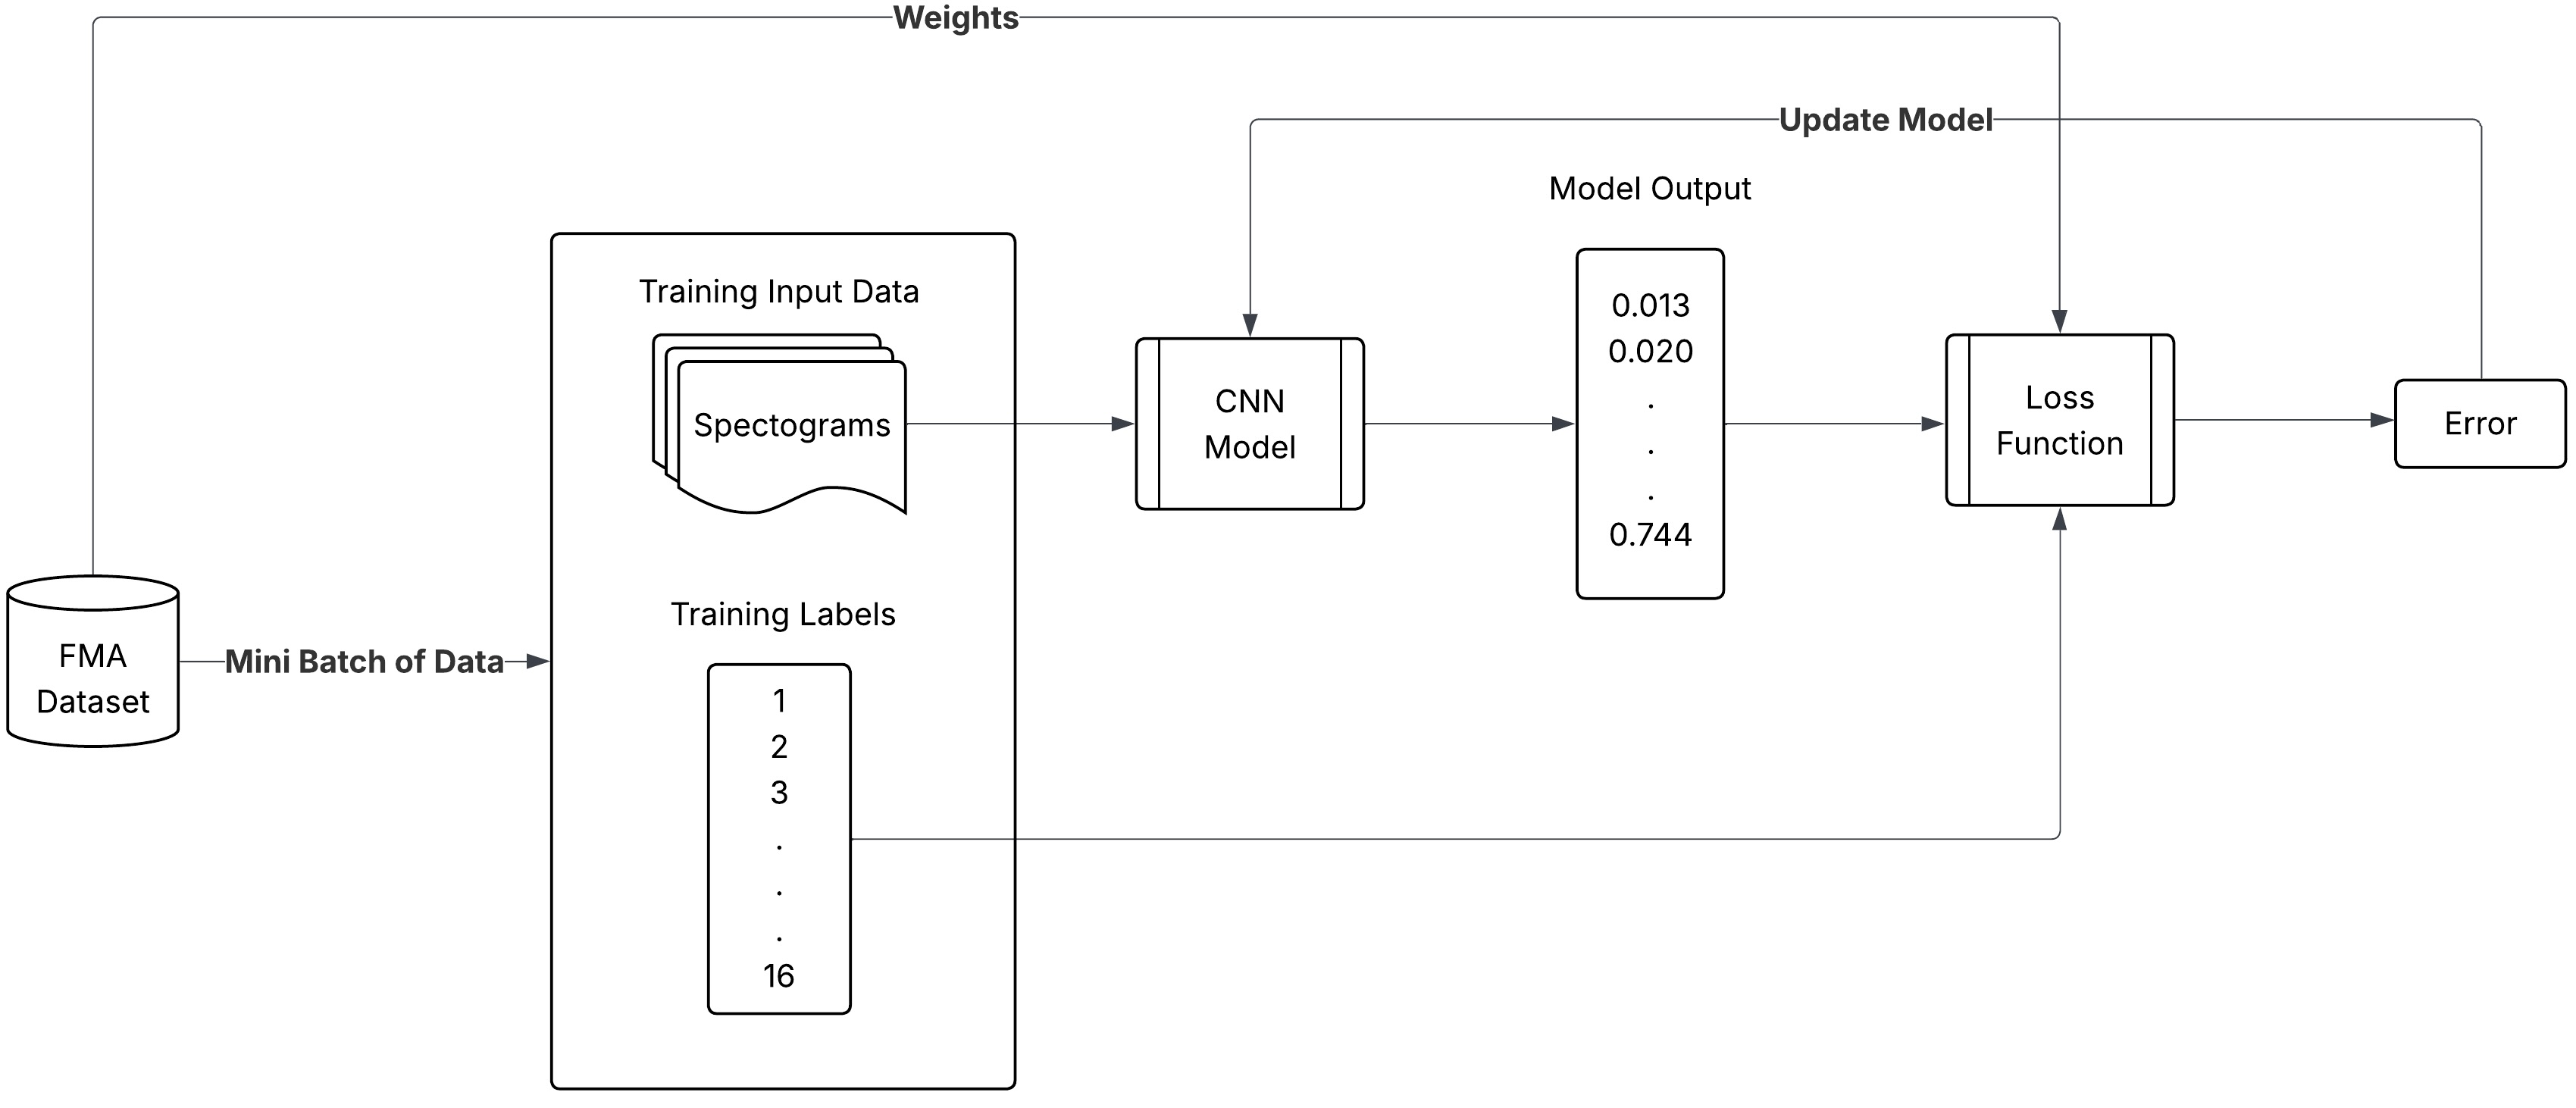
\includegraphics[width=0.9\textwidth]{model.jpeg}
  \caption{The components of the overall model}
  \label{fig:model_components}
\end{figure}

\section{Background \& Related Work}

Music genre classification is a well-researched area in the field of information retrieval. A music genre classification model can be used in music recommendation systems, auto-generated playlists, and market analysis, identifying popular genres for music producers.

As early as 2002, traditional machine learning approaches have been developed for music genre classification. Tzanetakis and Cook extracted features like timbral texture, pitch and rhythmic content from audio files before feeding them into traditional machine learning classifiers like KNN and Gaussian mixture models. They achieved a classification accuracy of 63\%, which was comparable to human performance at the time \citep{tzanetakis2002}. The dataset developed in the research was widely used in subsequent studies and is regarded as the famous GTZAN dataset.

Deep learning approaches later emerged in the 2010s. One such example is a convolutional recurrent neural network, which replaces the last layer of a CNN model with an RNN and has proven to be more effective than pure CNNs in music genre classification \citep{choi2017crnn}.

In 2025, Zhang and Li proposed a parallel CNN ensemble model that integrates three CNN models handling features from discrete wavelet transform, Mel frequency spectral coefficients, and short-time Fourier transform of audio files \citep{zhang2025ensemble}. As a result, they achieved a classification accuracy of 96.07\% on the GTZAN dataset.

In addition to academic advancements, music genre classification softwares also emerged in the market. One such example is Cyanite, which provides a comprehensive music sorting solution by automatically retrieving a song’s BPM, genre, emotion and key descriptions \citep{cyanite_ai}. Cyanite uses a similar approach to ours by converting audio files into spectrograms for inputs before generating descriptive tags based on perceived patterns.

Research in recent years has further advanced in deep learning approaches. In 2018, Oramas et al.\ proposed a multimodal approach, taking in audio, text reviews, and cover art pictures as input for music genre classification. The results showed that the combination of multiple modalities yields a higher accuracy than one modality in isolation \citep{oramas2018multimodal}. This opens the possibility of using multiple modes of data to train our model for genre classification to boost accuracy or mitigate bias across data.


\section{Data Processing}

The dataset we are using will be the Free Music Archive (FMA) dataset \citep{fma_dataset}. The full dataset contains 106,574 tracks with 16 different top-level genres and 161 sub-genres. However, the complete dataset is 879 gigabytes, which is too large to train with. The FMA Large subset will be used instead, which contains the same tracks trimmed down to 30-second snippets. Along with the dataset, the FMA repository includes a metadata folder listing all the songs and their corresponding genres, helping with data organization and classification.

Upon examining the metadata, not all songs had their genres labeled. After using the \texttt{pandas} Python package to remove all rows without labels, the dataset was reduced to approximately 50,000 tracks(see Table~\ref{tab:genre_counts} below for the genres available, and their track count). However, the genre distribution remained unbalanced, with only 7 genres containing over 2,000 tracks. Since our goal is to classify as many genres as possible, we will use a weighted loss function that penalizes the model more heavily when it fails to classify underrepresented genres to prevent overfitting on genres with more data \citep{tantai_weighted}. Since 12 genres have at least 400 tracks, we have decided to have a minimum and maximum of 400 and 2,500 tracks per genre, respectively, allowing us to have about 20,000 tracks to train our model with.

\begin{table}[h]
\centering
\caption{Track count by genre in the FMA dataset}
\label{tab:genre_counts}
\begin{tabular}{lr}
\toprule
\textbf{Genre} & \textbf{Track Count} \\
\midrule
Rock                & 14,182 \\
Experimental        & 10,608 \\
Electronic          & 9,372 \\
Hip-Hop             & 3,552 \\
Folk                & 2,803 \\
Pop                 & 2,332 \\
Instrumental        & 2,079 \\
International       & 1,389 \\
Classical           & 1,230 \\
Jazz                & 571 \\
Old-Time / Historic & 554 \\
Spoken              & 423 \\
Country             & 194 \\
Soul-RnB            & 175 \\
Blues               & 110 \\
Easy Listening      & 24 \\
\bottomrule
\end{tabular}
\end{table}


We will take the following steps to format the data:

\begin{enumerate}
    \item To select the tracks for each genre, you must iterate through the folders that contain the tracks using the \texttt{os} Python package.
    \item Compare the file names to the track IDs provided in the \texttt{tracks.csv} metadata file to obtain each song’s top genre.
    \item Add each specified song’s file path to a corresponding list based on its genre. 
    \item Use the \texttt{librosa} package to convert each song into a Mel spectrogram, which is a 2D time-frequency image suitable for training a CNN \citep{doshi_mel_spectrogram}.
    \item Convert each Mel spectrogram into PyTorch tensors and store them in respective lists by genre.
    \item Use the \texttt{scikit-learn} package to split each genre into 70\% training, 15\% validation, and 15\% testing using the \texttt{train\_test\_split()} function \citep{buhl_split}.
\end{enumerate}

To achieve the highest training accuracy with respect to the data, we will use Mel spectrograms with 512 frequency bands, similar to an experiment performed by Cheuk et al.\ \citep{cheuk2020impactaudioinputrepresentations}. This can be done by tuning the \texttt{n\_mels} hyperparameter in the \texttt{librosa} package. Although log-frequency constant-Q transforms (CQT) have shown higher accuracy in some cases, their significantly larger size (e.g., using 2,048 or 4,096 frequency bands) increases training costs without yielding proportionally better results in transcription accuracy \citep{cheuk2020impactaudioinputrepresentations}.


\section{Architecture}

The architecture for this model will be a CNN instead of a Recurrent Neural Network (RNN). This is because CNNs are generally better at detecting local features and processing input data simultaneously, making this neural network optimal for the spectrogram representation of songs \citep{kalra2023cnn_imageclass}. Based on a study done by Jiménez and José, CRNNs (which combine features of CNNs and RNNs) tend to overfit too quickly in comparison to CNNs, making training potentially unstable \citep{jimenez2020genre}. Furthermore, Dense Neural Networks (DNNs), despite being easier to train, lack the accuracy that CNNs can achieve, making them unsuitable as well \citep{landschoot2020github}.

The activation function for the model will be \( f(x) = -x \cdot \mathrm{erf}(e^{-x}) \), where \(\mathrm{erf}()\) is the Gaussian error function(see the linked Wikipedia page for more information) \citep{wikipedia_error_function}. This functionw as chose as it  outperformed current industry functions in 92.8\% of the 28 studied cases \citep{RAHMAN2024112502}. The optimizing function and classifying functions will use the Adam optimizer, as it is the current default choice for many CNNs \citep{rafalski2025cnnopt}. Finally, the loss function is the PEDCC-Loss combined with the AM-Softmax function, which achieved the highest accuracy across all experiments conducted by Zhu et al.\ \citep{DBLP:journals/corr/abs-1904-06008}.

Another proposed loss function to address bias within the dataset is to use a weighted Cross Entropy Loss (CEL) function, since there are some genres with fewer songs than others in the dataset. The weight for each genre will be calculated as the total number of samples divided by the number of samples in its respective genre. For example, out of 1,000 samples, “Class B” may have 800, so its weight would be \(1000 / 800 = 1.25\) \citep{tantai_weighted}.

The hyperparameters can be further optimized using the Modified Electric Eel Foraging Optimization algorithm (MEEFO). This algorithm allows the model to be trained more effectively and may be more beneficial than similar training algorithms like the Black Hole Optimization Algorithm (BHO). MEEFO avoids early solution convergence \citep{zhang2025zfnet}, allowing the model to explore more solutions and better optimize performance. The implementation of the model will follow the approach outlined by Maged et al.\ in Section 4 \citep{MAGED2024102855}.



\section{Baseline Model}

The baseline model will follow closely with the one developed by Landschoot et al.\ (2023) \citep{landschoot2020github}. The baseline model must be a multinomial regression model, since there are multiple genres of music to be classified \citep{jesussek2023logistic}. The original baseline model uses the LBFGS solver as the optimization function \citep{landschoot2020github}. 

The baseline model will be implemented using the \texttt{LogisticRegressionCV} function from \texttt{scikit-learn} \citep{scikit_learn_website}, where the \texttt{multi\_class} parameter is set to \texttt{"multinomial"} and the solver is \texttt{"lbfgs"}. This model is expected to achieve an accuracy of approximately 53\% \citep{landschoot2020github}, which serves as a useful benchmark to determine whether our implementation is consistent with previously reported outcomes.

\section{Ethical Concerns}

Mel spectrograms emphasize frequencies that are more aligned with how the human ear perceives sound \citep{landschoot2020github}. This means that different vocal tones, accents, or speech cadences that are common across different ethnic groups can appear as distinct frequency patterns. If a model is trained on a dataset where these patterns are consistently labeled under certain genres, such as deeper male voices or specific speech patterns being linked to rap or hip-hop, the model might start using these surface-level cues to make predictions. A song could therefore be classified as “rap” not because of its musical structure, instrumentation, or intent, but because of how the artist’s voice appears visually in the spectrogram. This introduces the risk of racial bias, as the model may reinforce stereotypes embedded in the training data. Over time, such a model could misrepresent artists: particularly those creating genre-bending work like Tyler the Creator’s \textit{Igor} album by categorizing them as rap despite the album’s diverse and cross-genre sound.

Another ethical concern lies in the dataset itself. The current dataset was selected primarily for its large volume of labeled examples; however, it consists predominantly of Western music genres. This imbalance may cause the model to generalize poorly on non-Western music, perpetuating a Western-centric bias in genre classification. To mitigate this, we will apply weighted loss functions that penalize misclassifications more heavily for underrepresented genres. This strategy aims to reduce overfitting to dominant classes and improve the model’s ability to generalize across a broader spectrum of musical traditions.


\section{Project Plan}

Our team will work remotely as one teammate is located in Australia. To organize effective collaboration across time zones, Discord is the primary source of communication. Depending on team availability, we plan to meet at least twice a week: once on either Saturday or Sunday, and once on Wednesday or Thursday. During these meetings, we will review progress, align our goals, and delegate upcoming tasks as we progress through the project. To ensure the code is not overwritten, Google Colab will be linked to GitHub for version control and branch management. See Table~\ref{tab:deliverables} below for the deliverables and deadlines assigned to each member. Attached is the \href{https://drive.google.com/drive/folders/1QGxYpoasWKFKUcYMxIBiFAGk11h4XRYb?usp=sharing}{Google folder} containing the Colab notebook, and the \href{https://github.com/TangALE/Music_Genre_Classification}{GitHub repository}.


\begin{table}[h]
\centering
\caption{Task delegation and expected timelines for each task}
\label{tab:deliverables}
\begin{tabular}{lll}
\toprule
\textbf{Deliverable} & \textbf{Deadline} & \textbf{Member} \\
\midrule
Team Formation & DONE & -N/A- \\
Project Proposal & June 13th & Everyone \\
Intro, Illustration & DONE & Josie \\
Background (4) & DONE & Allen \\
Data Processing, Risk Register & DONE & Ruian \\
Architecture, Baseline Model, Ethical Considerations & DONE & Daniel \\
Project Plan (4) & DONE & All members \\
Data Processing & June 20 & Ruian \\
MEEFO algo (hyperparameter tuning) & July 12 & Ruian \\
CNN Model (layers, activation function, optimizer function) & June 30 & Daniel \\
Testing against Baseline Model & July 12 & Allen \\
Creating a Baseline Model & June 30 & Allen \\
CNN Model Loss & June 30 & Josie \\
\bottomrule
\end{tabular}
\end{table}

\section{Risk Register}

\textbf{Colab Session Timeouts (High Likelihood):} \\
Colab sessions automatically time out after 12 hours, so we will checkpoint our model periodically (every hour or so) in case it times out during training. This way, the current weights and progress are saved, and significant work will not be lost when session timeouts occur. Preprocessing the data beforehand, prior to using Google Colab, will also save time and help avoid training interruptions.

\textbf{Team Member Drops Out/Emergency (Medium Likelihood):} \\
This situation may arise if a team member drops the course, experiences a family emergency, or is otherwise unable to complete their assigned work. We will manage the situation by dividing tasks evenly and setting internal deadlines at least three days ahead of the course deadlines. This buffer allows time to address availability issues and enables other team members to step in if needed. Furthermore, our twice-weekly meetings facilitate communication of any issues early on, helping us adapt and plan accordingly.

\textbf{Model Training Takes Too Long (High Likelihood):} \\
If the model takes too long to train, it may result in an incomplete or non-functional version by the end of the project. To mitigate this risk, we will start by training smaller models with fewer epochs and layers to test performance. This will allow us to gauge the minimum architectural requirements and apply additional optimizations such as spectrogram resizing or hyperparameter tuning to keep training time within acceptable limits.

\textbf{Genre Data Imbalance (High Likelihood):} \\
Several genres in our dataset contain fewer than 2,000 songs, while others have over 10,000. This imbalance could cause the model to overfit to the dominant genres and fail to generalize well. To address this, we apply a weighted loss function that penalizes the model more heavily for misclassifying underrepresented genres \citep{tantai_weighted}.



\label{last_page}

\bibliography{APS360_ref_cleaned}
\bibliographystyle{iclr2022_conference}

\end{document}
